\title{MIUP'2014}

\documentclass[11pt]{report}
\usepackage[utf8]{inputenc}
\usepackage[T1]{fontenc}
\usepackage{graphicx}
\usepackage{url}
\usepackage{fancyhdr}
\usepackage{lastpage}
\usepackage{multicol}
\usepackage{fullpage}
\usepackage{wrapfig}
\usepackage{hyperref}
\usepackage[margin=0.80in]{geometry}

\begin{document}

\begin{titlepage}
\begin{center}
\vspace*{2.5in}

\includegraphics[width=1.0\textwidth]{LOGO_withSponsors.png}~\\[1cm]
\texttt{http://miup2014.github.io/}
\end{center}
\end{titlepage}

\tableofcontents
\clearpage

\section*{Local Organizers}

\begin{itemize}
\item Hugo Sereno Ferreira, FEUP (Chair)
\item João Azevedo, ShiftForward
\item Luís Fonseca, ShiftForward
\item Miguel Oliveira, FEUP
\item Tiago Boldt Sousa, FEUP
\end{itemize}

\section*{Scientific Committee}

\begin{itemize}
\item André Restivo (Universidade do Porto - FEUP)
\item Fábio Marques (Universidade de Aveiro)
\item Hugo Sereno Ferreira (Universidade do Porto - FEUP)
\item Luís Paquete (Universidade de Coimbra)
\item Margarida Mamede (Universidade Nova de Lisboa)
\item Miguel Oliveira (Universidade do Porto - FEUP)
\item Paulo Crocker (Universidade da Beira Interior)
\item Pedro Guerreiro (Universidade do Algarve)
\item Pedro Mariano (Universidade de Lisboa)
\item Pedro Rangel Henriques (Universidade do Minho)
\item Pedro Ribeiro (Universidade do Porto - FCUP)
\item Rui Mendes (Universidade do Minho)
\item Vasco Pedro (Universidade de Évora)
\end{itemize}

\section*{Student Volunteers}

\begin{itemize}
\item Diogo Santos (MIEIC)
\item João Correia Pinto (MIEEC)
\item João Maia (MIEIC)
\item João Pedro Dias (MIEIC)
\item José Pedro Pinto (MIEIC)
\item Tiago Simões Almeida (MIEM)
\item Tomás Tavares (MIEEC)
\end{itemize}

\section*{Compilation}

\begin{tabular}{| l | l | l | l | l |}
\hline
\textbf{Language} & \textbf{Extension} & \textbf{Compiler} & \textbf{Version} & \textbf{Compilation command} \\
\hline
\textbf{C} & .c & gcc & 4.6.4 & gcc -std=gnu99 -static \$file -lm \\
\textbf{C++} & .cpp & g++ & 4.6.4 & g++ -std=gnu++0x -static \$file \\
\textbf{Java} & .java & Java SE & 1.7.0\_67 & javac -encoding UTF-8 -sourcepath . -d . \$file \\
\hline
\end{tabular}

\section*{Compilation Constraints}

\begin{itemize}
\item \textbf{Maximum compilation time:} 60 seconds
\item \textbf{Maximum source code size:} 100 KB
\item Every source code must be submitted in a single file
\item In case of Java submissions, the .java file has to have the same name as the class that contains
  the main method. There is no limit for the number of classes contained in that file
\end{itemize}

\section*{Execution}


\begin{tabular}{| l | l |}
\hline
\textbf{Language} & \textbf{Execution command} \\
\hline
\textbf{C} & ./a.out \\
\textbf{C++} & ./a.out \\
\textbf{Java} & java -Xmx256M -Xss256M -classpath . \$name \\
\hline
\end{tabular}

\section*{Runtime constraints}

Unless \textbf{explicitly stated otherwise in the problem} the following limits
apply to all problems.

\begin{itemize}
\item \textbf{Maximum CPU time:} 1 second
\item \textbf{Maximum Memory:} 256MB
\end{itemize}

\section*{Formatting}

\begin{itemize}
\item All lines (both in the input and output) should be ended by the newline
  character (\texttt{'\textbackslash n'})
\item Except when explicitly stated, single spaces are used as a separator.
\item No line starts or ends with any kind of whitespace.
\end{itemize}

\section*{Documentation}

Language documentation is available, namely:
\begin{itemize}
\item man pages for C/C++ (using the command line)
\item C++ STL documentation (\url{http://184.73.172.95/STL_doc/})
\item Java SE 7 documentation (\url{http://184.73.172.95/JAVA_doc/})
\end{itemize}

\clearpage

\section*{Problem A: Water Point}
\addcontentsline{toc}{section}{Problem A: Water Point}

Forest fires are one of the main scourges plaguing countries during periods of greater heat. When fighting a fire, it is essential that fire vehicles being used (i.e., trucks, helicopters, planes) can be refilled in the shortest time possible.
For this purpose several water points (places where vehicles can refill their
tanks) are identified in the terrain. Due to their dimensions and overall
conditions not all water points are suited to fill the tanks of all types of
vehicles.

\subsection*{Task}

Help the fire fighters to determine which is the nearest suitable water point to fill the fire fighting vehicle. Helicopters and planes move in straight lines to reach the water points. You may consider that fire trucks can reach the water points moving along horizontal and/or vertical lines.

\subsection*{Input}

The first line identifies the type $t$ of the vehicle that needs to be refilled
(T for Truck, H for Helicopter, and P for Plane). The second line has the $x$
and $y$ coordinates (separated by a space) corresponding to the location of this
vehicle. The third line contains the number $n$ of existing water
points. Finally, the remaining $n$ lines have a number $i$ identifying the water
point, the water point $x_i$ and $y_i$ coordinates ($x_i$ and $y_i$ are integers
separated by a space) and the discrimination of all the types $t_i$ of vehicles that are able to refill their tanks in the water point ("T", "TH", or "THP"), all separated by a space. %If a water point is identified of type T, then it can only refill autotanks, if it is identified with an H (then both autotanks and helicopters can use the water point to refill). Finally, if it is identified with an A, then all vehicles can be refilled in that water point.

\subsection*{Constraints}

\begin{itemize}
        \item $t \in $ \{T, H, P\}
        \item $0 \leq i \leq 1000000$
        \item $1 \leq n \leq 100000$
        \item $0 \leq x, y, x_i, y_i \leq 1000000$
        \item $t_i \in $ \{T, TH, THP\}
\end{itemize}

\subsection*{Output}

The output is composed by a single line with the identifier $i$ of the nearest water point. If the vehicle is at the same distance from two or more water points, select the one with the smallest identifier $i$.

\subsection*{Input example 1}

\begin{verbatim}
H
10 10
5
5 30 60 T
1 50 50 THP
4 1 1 TH
3 3 15 TH
2 11 10 T
\end{verbatim}

\subsection*{Output example 1}

\begin{verbatim}
3
\end{verbatim}

\subsection*{Input example 2}

\begin{verbatim}
T
10 7
13
13 2 12 THP
9 11 8 TH
0 14 10 T
10 0 8 THP
3 11 3 THP
5 8 11 TH
2 2 4 TH
7 2 12 T
8 7 4 T
1 11 7 THP
11 12 13 TH
6 11 9 TH
12 0 8 T
\end{verbatim}

\subsection*{Output example 2}

\begin{verbatim}
1
\end{verbatim}

\clearpage

\section*{Problem B: Chaotic Stock Exchange}
\addcontentsline{toc}{section}{Problem B: Chaotic Stock Exchange}

A stock market receives two kinds of orders: \emph{limit} and
\emph{market}. A \emph{limit order} is characterised by a tuple $(t,
q, p)$, where $t$ is its type (\emph{buy} or \emph{sell}), $q$ is the
quantity of stocks to trade and $p$ is the transaction price. A
\emph{market order} is characterised by a tuple $(t, q)$, where $t$ is
its type (\emph{buy} or \emph{sell}) and $q$ is the quantity of stocks
to trade. Limit orders are not processed right away when they arrive
in the stock market, whereas market orders are processed the moment
they arrive.

A \emph{buy limit order} means someone wants to buy stocks at a
certain price. When it arrives in the stock market it is inserted in a
\emph{buy limit order book}. When a \emph{sell market order} arrives
in the stock market, one of the buy limit orders with the highest
price in the buy limit order book is removed from the book and a
transaction is made. If there are still stocks in the market order to
be sold, the next buy limit order is removed until all stocks are
sold. The last buy limit order may reenter the limit order book if it
was only partially fulfilled by the last remaining stocks in the
market order. After processing, the stock price is set to the price of
the last buy limit order. If the orders in the limit order book do not
cover the market order, then the market order is discarded and the
stock value remains unchanged.

\emph{Sell limit orders} and \emph{buy market orders} are processed in
a similar way, with the sell limit orders going into the \emph{sell
  limit order book} and those with the lowest selling price having
precedence over the others. As with the buy limit orders, the last
sell limit order used to complete a buy market order determines the
stock price.

The behaviour of a stock value can be chaotic depending on the
properties of buy and sell orders. If a buy order has more stocks or a
lower price, the final stock value may be different, after processing
a batch of orders.

\subsection*{Task}

Given a batch of orders, by the order in which they arrived in the
stock market, your task is to determine the price of the stock after
all the orders have been processed.


\subsection*{Input}

The first line contains the number of orders in the batch, $N$, and
the initial stock value, $P_0$. The following $N$ lines contain either
one of:
\begin{itemize}
\item The character \verb|L|, followed by either an \verb|S| for a
  sell \emph{limit order} or a \verb|B| for a buy \emph{limit order},
  followed by the number of stocks to trade, and a number specifying
  the price.
\item The character \verb|M|, followed by either an \verb|S| for a
  sell \emph{market order} or a \verb|B| for a buy \emph{market
    order}, and the number of stocks to transact.
\end{itemize}
All the elements in a line are separated by one white space character.

\subsection*{Constraints}

$0 < N \le 100000$

\subsection*{Output}

The output contains a single number: the stock final price.

\subsection*{Input example 1}

\begin{verbatim}
11 2
L S 100 12
L S 100 13
L S 100 11
L B 100 9
L B 100 8
L B 100 10
M B 101
M S 201
M S 50
M B 51
M B 49
\end{verbatim}

\subsection*{Output example 1}

\begin{verbatim}
13
\end{verbatim}

\subsection*{Input example 2}

\begin{verbatim}
10 2
L S 100 12
L S 100 13
L S 100 11
L B 100 9
L B 100 8
L B 100 10
M B 301
M S 301
L S 100 7
L B 100 19
\end{verbatim}

\subsection*{Output example 2}

\begin{verbatim}
2
\end{verbatim}

\clearpage

\section*{Problem C: Team Formations}
\addcontentsline{toc}{section}{Problem C: Team Formations}

\begin{wrapfigure}{r}{0.35\textwidth}
  \centering
  \vspace{-15pt}
  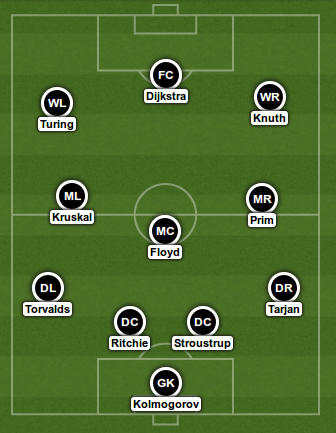
\includegraphics[width=0.35\textwidth]{tactics.png}
\end{wrapfigure}

Mr. John ``The Master'' Doe is the coach of CSFC (Computer Science
Football Club), the new shining star in world's football. John is very
worried about which tactics he should use. Should he play with a team
formation of 4-3-3, or should he go with a classical 4-4-2? Thinking
about it, he saw that there were many more possible formations!

In football there are 11 players in the field. One of them is the
goalkeeper and the other 10 players are traditionally distributed on
the field along three major roles: defenders,
midfielders and forwards. John is certain that he wants at least 3
defenders, at least 2 midfielders, and at most 3 forwards. Picking up a
piece of paper, he quickly saw that there were 18 possible
formations respecting these conditions:

\begin{verbatim}
3-4-3   3-5-2   3-6-1   3-7-0   4-3-3   4-4-2
4-5-1   4-6-0   5-2-3   5-3-2   5-4-1   5-5-0
6-2-2   6-3-1   6-4-0   7-2-1   7-3-0   8-2-0
\end{verbatim}

John thought about how this counting could be done for other
conditions and even for other sports, with a different number of
players and roles. Can you help him?

\subsection*{Task}

Given a number of players {\bf P}, a number of roles {\bf R}, and a
series of conditions indicating, for each role, a minimum or maximum
number of players, your task is to determine how many valid formations
exist, that is, using all the players and obeying the given conditions.

\subsection*{Input}

The first line of input contains a single number {\bf P}, the number of players.

The second line contains a single number {\bf R}, the number of roles
to consider. The next {\bf R} lines describe the conditions for each
role, with the $i$-th line describing the condition for role $i$. Each
of these lines comes in the format {\tt MIN X} (the respective role
must have at least $X$ players) or {\tt MAX X} (the respective role
must have at most $X$ players). $X$ is always larger or equal than
zero and smaller or equal than {\bf P}.

For better understanding, note that the first example input
corresponds to the example given in the problem statement, with 18
possible formations.

\subsection*{Output}

The output is a line containing the number of valid team formations
using all the players and respecting the conditions, that is, the
number of ways to distribute the players among the roles while not
breaking any of the given restrictions.

It may be the case that there are no team formations respecting the
conditions, in which case your answer should be zero. It is also
guaranteed that, for the given inputs, the result will fit in a normal
signed 64 bit integer.

\subsection*{Constraints}

\begin{tabular}{ l l }
$1 \leq {\bf P} \leq 50$   & Number of players \\
$1 \leq {\bf R} \leq 20$   & Number of team roles
\end{tabular}

\subsection*{Input example 1}
\begin{verbatim}
10
3
MIN 3
MIN 2
MAX 3
\end{verbatim}

\subsection*{Output example 1}
\begin{verbatim}
18
\end{verbatim}

\subsection*{Input example 2}
\begin{verbatim}
12
4
MAX 4
MIN 2
MAX 3
MIN 1
\end{verbatim}

\subsection*{Output example 2}
\begin{verbatim}
130
\end{verbatim}

\subsection*{Input example 3}
\begin{verbatim}
8
3
MIN 3
MIN 3
MIN 3
\end{verbatim}

\subsection*{Output example 3}
\begin{verbatim}
0
\end{verbatim}

\clearpage

\section*{Problem D: Cutting Metal Sheets}
\addcontentsline{toc}{section}{Problem D: Cutting Metal Sheets}

Metalworking is all about producing metal sheets for car bodies, roofs of buildings and airplane wings.
Ideally, these metal sheets should have no defective spot. However, it is not always possible
to obtain such perfect metal sheets out from the roll slitting machine.\\

Nowadays, defective stops are almost not visible, but they can still affect the properties of the metal sheet.
Depending of the application, a certain number of defective spots may be allowed.\\

\begin{wrapfigure}{r}{0.5\textwidth}
  \centering
  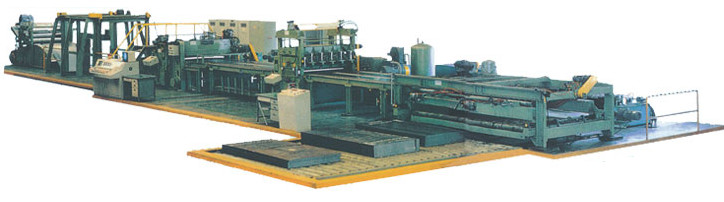
\includegraphics[width=0.5\textwidth]{roll}
  \caption{A roll slitting machine.}
\end{wrapfigure}

The overall process works as follows: A quantity of metal that is larger than required, is used produce an over-sized rectangular
sheet of metal. The coordinates of defective spots from the sheet of metal are detected by a computer vision equipment.
Then, a smaller sheet is cut such that it does not contain more than a given number of defective spots, which has been defined
by the worker. Of course, in order to avoid waste, this smaller sheet of metal should be as large as possible.\\

\subsection*{Task}

Implement an algorithm that cuts the largest axis-aligned rectangular sheet of metal
that has at most $K$ defective spots.

\subsection*{Input}

The input may consist of several test cases. The first line of each test case
gives the $x$ and $y$ (integer) coordinates of the lower-left and
upper-right corners of the larger sheet of metal, which may range from $0$ to $30000$,
separated by white space. Then, the number of defective spots, $N$,
as well as the maximum number of allowed defective spots, $K$, is
given in the second line. The following $N$ lines provide the $x$ and
$y$ coordinates of the spots, one spot per line.
A new test case may follow in the next line.\\

Note that different spots always differ in both coordinates.
In addition, consider that a sheet of metal
that is cut in a spot does not contain that spot.

\subsection*{Output}

The output of each test case is the area of the rectangular sheet of paper.

\subsection*{Constraints}
\begin{tabular}{ l l }
$0 \leq {\bf N} \leq 500$      & Number of defective spots \\
$0 \leq {\bf K} \leq 50$        & Number of allowed defective spots \\
$0 \leq {\bf R} \leq 30000$     & Range of coordinates.
\end{tabular}\\\bigskip

There are at most 2 test cases in a single file.\\\medskip

The time limit is 2 seconds.

\subsection*{Input example}

\begin{verbatim}
20 10 1000 500
10 5
33 221
714 222
803 350
805 67
745 33
949 213
328 392
581 429
980 104
769 332
20 10 1000 500
10 1
33 221
714 222
803 350
805 67
745 33
949 213
328 392
581 429
980 104
769 332
\end{verbatim}

\subsection*{Output example}

\begin{verbatim}
396628
285339
\end{verbatim}

\clearpage

\section*{Problem E: Checking Quality}
\addcontentsline{toc}{section}{Problem E: Checking Quality}

Tony is very excited. He just started a new job as a software engineer. As a
starter project, he is getting acquainted with his team’s supervised machine
learning system. After training the system, the testing data results are
compared to the expected (known) outcome. For each testing example, the system
produces a confidence value in the classification and the result is either:

\begin{itemize}
\item Classified correctly, meaning that the result matched the expected one.
\item Classified incorrectly, meaning that the result was different than the expected one.
\end{itemize}

Given a value \textbf{W}, the system only decides to actually make a
classification if its confidence in the classification is greater than
\textbf{W}. Tony needs to assess the quality of the results. For this, he wants
to calculate both the precision and the recall of the system.

\begin{itemize}
\item Precision is the number of correct classifications divided by the total
  number of produced classifications.
\item Recall is the number of correct classifications divided by the number of classifications that should have been made.
\end{itemize}

Tony is having difficulties in calculating the best \textbf{W}, in order to
maximize the system precision and recall. Can you help him out?

\subsection*{Problem}

Given a set of \textbf{N} classifications and \textbf{Q} possible confidence values, find the the total number of classifications and correct classifications for each confidence value.

\subsection*{Input}

The first line contains \textbf{N} ($1 \leq \textbf{N} \leq 100000$), the number
of classifications. The next \textbf{N} lines contain the description of each
classification: an integer $\mathbf{C}_i$ ($0 \leq \mathbf{C}_i \leq 10^9$),
representing the confidence in the output, and the classification result.

A line with an integer \textbf{Q} ($1 \leq \textbf{Q} \leq 100000$) follows, the
number of possible confidence values. Then \textbf{Q} lines, each with an
integer $\mathbf{W}_i$ ($1 \leq \mathbf{W}_i \leq 10^9$).

\subsection*{Output}

For each query, output a line for each query with two space separated integers: the number of classifications and the number of correct classifications with confidence higher than $\mathbf{W}_i$.

\subsection*{Sample Input}

\begin{verbatim}
4
8 Classified correctly
2 Classified incorrectly
5 Classified incorrectly
1 Classified correctly
2
3
7
\end{verbatim}

\subsection*{Sample Output}

\begin{verbatim}
2 1
1 1
\end{verbatim}

\clearpage

\section*{Problem F: Financial Wizards}
\addcontentsline{toc}{section}{Problem F: Financial Wizards}

Supercalifragilistic Bank has developed a new financial product and is eager to sell this product to clients willing to invest. The financial product, called the Golden Lattice, is based on a new and extremely cunning investment strategy  that relies on a specific and predictable revenue income from the investors; the banks fund managers claim to have found exciting new investment strategies exploiting this fact. Investors are required to make monthly payments into the fund where the next payment is a sum of the two previous payments,  more precisely it's the sum of the previous months payment plus double the value of the payment two months previously.

The Bank of Portugal has of course already detected a possible flaw in this product and prohibited any \textit{negative} initial investment and insisted that all the payments into the fund must be positive.

\subsection*{Task}

The initial two monthly payments are capped at a maximum value of 100,000 Euros. Also the bank requires that a monthly payment be at least as big as the previous months payment.  Investors simply state the number of months they wish to invest  and the last value they wish to invest.

Your job is to  to simply calculate the first two initial payments. For instance if the last payment is 169 Euros and the duration is 6 months then the first two payments are 2 and 5 euros respectively (hence the third payment will be 12 euros).

In order for the product to be lucrative for the bank the duration the clients must make payments between one and two years.
% 2 5 12 29 70 169

\subsection*{Input}
The input consists of two lines. The first line is the duration of the product (12-24 months). The second line contains the value of the final payment into the fund.

\subsection*{Constraints}
The last payment will not exceed 2000 million Euros.
For the given test cases there exists a unique solution (the two initial values) to the problem or no solution whatsoever.

\subsection*{Output}
A single line with two integer values (the first and the second payments) separated by a space or the string \textit{"No Solution"} when it is not possible to have two first payments obeying the conditions.

\subsection*{Sample Input}
\begin{verbatim}
16
196721422
\end{verbatim}
\subsection*{Sample Output}
\begin{verbatim}
21 1000
\end{verbatim}
\subsection*{Sample Input}
\begin{verbatim}
23
964212436
\end{verbatim}
\subsection*{Sample Output}
\begin{verbatim}
No Solution
\end{verbatim}

\clearpage

\section*{Problem G: Ryanware}
\addcontentsline{toc}{section}{Problem G: Ryanware}

\begin{wrapfigure}{r}{0.5\textwidth}
  \centering
  
\includegraphics[width=0.5\textwidth]{ryanware}
\end{wrapfigure}

Luckily for all of us, the popular low-cost airline \textit{Ryanware} now offers the possibility of free seat reservation. Until a few  months ago, if you wanted to reserve a seat, and not have to fight for it upon entering the plane, you would have to pay.

Notwithstanding, please understand that \textit{Ryanware} chooses the seat that it reserves for you. If you want to pick a specific seat on the plane, you may, but then you have to pay. Using the free reservation system, you get what appears to be a randomly allocated seat.

Actually, the seats are not allocated randomly. There are very specific rules.

\subsection*{Task}

Your task is to write the program that will perform the seat reservation for \textit{Ryanware}, given the current occupation of the plane and the number of seats to reserve together. In fact, if you reserve say, four seats, the system will understand that that is a family (or a group of friends) and will try to seat them together.

All \textit{Ryanware} planes are equal. The passenger cabin has a number of
rows, and each row has six seats: three on the left bench and three on the right
bench. In each row, seats are identified by a letter, from \textit{A} to
\textit{F}. Seats \textit{A}, \textit{B} and \textit{C} are on the left bench
and seats \textit{D}, \textit{E} and \textit{F} are on the right bench. More
precisely, \textit{A} is the window seat on the left and \textit{F} is the
window seat on the right; \textit{B} is the middle seat on the left and
\textit{E} is the middle seat on the right; \textit{C} is the aisle seat on the
left and \textit{D} is the aisle seat on the right.

If you are a solo traveller, reserving only one place, you will get the window
seat in the frontmost bench that is currently empty. If there are no empty
benches, but there are benches having adjacent empty seats, you will get the
seat in the frontmost such bench, that is not next to the occupied seat on the
same bench (meaning a free seat is left between you and your neighbour). If no
benches with adjacent empty seats remain, but there are benches with two empty
seats (the center seat is taken), you will get the window seat on the frontmost
such bench. If all benches have at most one free seat, you will get that free
seat in the frontmost such bench.

In this description, “frontmost” means as close as possible to the front of the
plane, which translates to the least possible row number. In case of a tie, that
is, if possible seats exists on the both benches of the same frontmost row, we
always prefer the leftmost bench. This applies to the following rules too.

If you are travelling with one friend, and you are trying to reserve two places together, the rules are similar: you will get the window seat and the middle seat in the frontmost bench that is currently empty. If there are no empty benches, but there are benches having two adjacent empty seats, you will get those two seats in the frontmost such bench. If this is not possible, the rule for solo travellers will be used twice, and you will probably seat away from your friend.

If you are travelling with two friends, and want to reserve three places together, the rules are similar again: you will get the three seats in the frontmost bench that is currently empty. If no benches are empty, the rule for pairs is used for two of you and then the rule for solo traveller is used for the third one.

If you want to reserve four places together, the system will use the rule for pairs twice (and it may happen that two of you will seat in the front the plane and the other two in the back…)

If you want to reserve \textbf{N} places, for $\textbf{N} \geq 5$, the system applies the above rules, first for 3 places, and then recursively for $\textbf{N}-3$ places.

These rules mean that if you are travelling in a big group, the sooner you
reserve the higher is the likelihood of sitting together.

\subsection*{Input}

The first line of the input file contains one number, \textbf{R}, representing the number of rows in the plane.
The second line contains one number, \textbf{S}, representing the number of seats that have already been reserved.
\textbf{S} lines follow, representing the seats that have been reserved. Each of
these lines contains one number, \textbf{X}, and one uppercase letter, \textbf{Y},
separated be a space. The number represents the seat row, and the letter
represents the seat letter, in the usual airline convention, explained above.

Another line follows, which contains one number, \textbf{Q}, representing the
number of parties making reservations. A party is a group of people reserving
together. \textbf{Q} lines follow. Each of these \textbf{Q} lines contains a
number $\mathbf{N}_i$, for \textbf{i} in 1 to \textbf{Q}, representing the
number of people in the \textbf{i}-th party.

\subsection*{Output}

The output file shall contain \textbf{Q} lines, one line for seats of each reservation.
More precisely, line \textbf{i}, for \textbf{i} in 1 to \textbf{Q}, contains the
list of seats that were allocated to the \textbf{i}-th party. The seats are
written using the same format as the input file, each separated from the next by
one space and in lexicographically order.

\subsection*{Restrictions}

\begin{itemize}
\item Number of rows, \textbf{R}: $2 \leq \textbf{R}$ and $\textbf{R} \leq 1000$
\item Number of reserved seats, \textbf{S}: $0 \leq \textbf{S}$ and $\textbf{S} < \textbf{R} * 6$
\item Row number, \textbf{X}: $1 \leq \textbf{X}$ and $\textbf{X} \leq \textbf{R}$
\item Seat letter, \textbf{Y}: either ‘A’, ‘B’, ‘C’, ‘D’, ‘E’, or ‘F’
\item Size of each party, $\mathbf{N}_i$: $0 < \mathbf{N}_i$, for \textbf{i} in 1 to \textbf{Q}
\item Total seats reserved: $\mathbf{N}_1 + \mathbf{N}_2 + … +
  \mathbf{N}_Q + \textbf{S} \leq \textbf{R} * 6$
\end{itemize}

\subsection*{Observation}

Note that some of the seats marked as reserved in the input file may have been
reserved using other rules. For example, a solo traveller, having made a payed
reservation in an empty plane, may have chosen an aisle seat.

\subsection*{Example Input}

\begin{verbatim}
4
6
1 B
3 B
2 A
2 D
2 E
2 F
5
1
4
5
3
2
\end{verbatim}

\subsection*{Example Output}

\begin{verbatim}
1 F
3 E 3 F 4 A 4 B
1 D 1 E 4 D 4 E 4 F
1 A 2 B 2 C
1 C 3 A
\end{verbatim}

\clearpage

\section*{Problem H: Hard Weeks}
\addcontentsline{toc}{section}{Problem H: Hard Weeks}

A well-known high-tech company is starting a huge project.
% with thousands of small tasks.
A detailed plan has already been done:
it contains all tasks to be undertaken and
specifies the precedence relation among them.
Each task takes exactly one week to be performed.
In order to shorten the duration of the whole project,
every task will start as soon as possible,
that is,
immediately after all precedent tasks have been completed.
Consequently, there may be weeks with several tasks to carry out.
If the number of tasks to be performed in a single week is
above a given \textit{limit},
that week will be \textit{hard} to everyone.
So, employees want to know
the maximum number of tasks to be performed in a single week and
how many hard weeks will come.

In the project whose plan is depicted in the figure,
there are $12$ tasks.
An arrow from task $t_1$ to task $t_2$ means that
$t_1$ has to be concluded before $t_2$ starts.
\begin{center}
\begin{picture}(440,100)(0,0)
%\put(  0,  0){\framebox(440,100){}}
\thicklines
\put( 60, 80){\begin{picture}(30,30)
              \put(   0,  0){\makebox(20,20){$0$}}
              \put(  10, 10){\circle{20}}
              \put( 2.5, 2.5){\vector(-3,-2){42.5}}
              \put(17.5, 2.5){\vector( 3,-2){42.5}}
              \end{picture}}
\put(180, 80){\begin{picture}(30,30)
              \put(  0, 0){\makebox(20,20){$1$}}
              \put( 10,10){\circle{20}}
              \put(  0,10){\vector( -1, 0){99}}
              \put( 2.5, 2.5){\vector(-3,-2){42.5}}
              \put(17.5, 2.5){\vector( 3,-2){42.5}}
              \end{picture}}
\put(300, 80){\begin{picture}(30,30)
              \put(  0, 0){\makebox(20,20){$2$}}
              \put( 10,10){\circle{20}}
              \end{picture}}
\put(  0, 40){\begin{picture}(30,30)
              \put(  0, 0){\makebox(20,20){$5$}}
              \put( 10,10){\circle{20}}
              \put(17.5, 2.5){\vector( 3,-2){42.5}}
              \end{picture}}
\put(120, 40){\begin{picture}(30,30)
              \put(  0, 0){\makebox(20,20){$6$}}
              \put( 10,10){\circle{20}}
              \put( 20,10){\vector( 1, 0){99}}
              \end{picture}}
\put(240, 40){\begin{picture}(30,30)
              \put(  0, 0){\makebox(20,20){$7$}}
              \put( 10,10){\circle{20}}
              \put(17.5,17.5){\vector( 3, 2){42.5}}
              \put(17.5, 2.5){\vector( 3,-2){42.5}}
              \end{picture}}
\put( 60,  0){\begin{picture}(30,30)
              \put(  0, 0){\makebox(20,20){$8$}}
              \put( 10,10){\circle{20}}
              \put(17.5,17.5){\vector( 3, 2){42.5}}
              \put( 20, 10){\vector( 1, 0){219}}
              \end{picture}}
\put(300,  0){\begin{picture}(30,30)
              \put(  0, 0){\makebox(20,20){$9$}}
              \put( 10,10){\circle{20}}
              \end{picture}}

\put(360, 80){\begin{picture}(30,30)
              \put(  0, 0){\makebox(20,20){$3$}}
              \put( 10,10){\circle{20}}
              \end{picture}}
\put(420, 80){\begin{picture}(30,30)
              \put(   0,  0){\makebox(20,20){$4$}}
              \put(  10, 10){\circle{20}}
              \put( 2.5, 2.5){\vector(-2,-3){43.5}}
              \put(  10,  0 ){\vector( 0,-1){59.1}}
              \end{picture}}
\put(360,  0){\begin{picture}(30,30)
              \put(  0, 0){\makebox(20,20){$10$}}
              \put( 10,10){\circle{20}}
              \put( 10,20 ){\vector( 0, 1){59.1}}
              \end{picture}}
\put(420,  0){\begin{picture}(30,30)
              \put(  0, 0){\makebox(20,20){$11$}}
              \put( 10,10){\circle{20}}
              \end{picture}}
\end{picture}
\end{center}
The tasks to carry out in each week are shown in the table below.
The maximum number of tasks to be performed in a single week is \textbf{3}
(tasks $0$, $10$ and $11$ in the second week).
Besides,
if the definition of hard week was a week with more than \textbf{1} task,
there would be \textbf{4} hard weeks
(the first three weeks and the last one).
\begin{center}
\begin{tabular}{|c|c|c|}                              \hline
\textbf{Week} & \textbf{Tasks}\\  \hline
{\bf 1} & $1$ and $4$        \\ \hline
{\bf 2} & $0$, $10$ and $11$ \\ \hline
{\bf 3} & $3$ and $5$        \\ \hline
{\bf 4} & $8$                \\ \hline
{\bf 5} & $6$                \\ \hline
{\bf 6} & $7$                \\ \hline
{\bf 7} & $2$ and $9$        \\ \hline
\end{tabular}
\end{center}


\subsection*{Task}

Given a (consistent) plan of the project
(with its tasks and the precedence relation among them) and
a number $L$ of tasks,
the goal is to find out
the maximum number of tasks to be performed in a single week and
the number of hard weeks
(i.e., the number of weeks with more than $L$ tasks to carry out).


\subsection*{Input}

The first line of the input has three integers: $T$, $P$, and $L$.
$T$ is the number of tasks,
$P$ is the number of (distinct) direct precedences among tasks, and
$L$ is the limit used in the definition of hard week.
Tasks are identified by integers, ranging from $0$ to $T-1$.

Each of the following $P$ lines contains two different integers,
$t_1$ and $t_2$,
which indicate that task $t_1$ has to be completed before task $t_2$ starts.

Integers in the same line are separated by a single space.


\subsection*{Constraints}

\begin{tabular}{ll}
$2 \leq T \leq  5\,000$ & Number of tasks.              \\
$1 \leq P \leq 300\,000$ & Number of direct precedences. \\
$1 \leq L < T$ & Limit used in the definition of hard week.
\end{tabular}


\subsection*{Output}

The output has a single line with two integers,
separated by a single space,
which are
the maximum number of tasks to be performed in a single week and
the number of hard weeks, respectively.
%(i.e., the number of weeks with more than $L$ tasks to carry out).



\subsection*{Input example}

\begin{verbatim}
12 14 1
0 5
0 6
1 0
1 6
1 7
7 2
5 8
8 9
10 3
8 6
4 10
7 9
4 11
6 7
\end{verbatim}

\subsection*{Output example}

\begin{verbatim}
3 4
\end{verbatim}

\clearpage

\section*{Problem I: Gazing Into the Past}
\addcontentsline{toc}{section}{Problem I: Gazing Into the Past}

Instead of gazing at crystal balls, archeologists study ancient
artifacts, with the hope that they will reveal the secrets of the life
of long gone civilisations. One important kind of such artifacts are
inscriptions, often engraved in stone, which may provide a wealth of
information on the people who left them.
% Archeologists even manage to consider things like laundry lists
% interesting\ldots

\begin{center}
  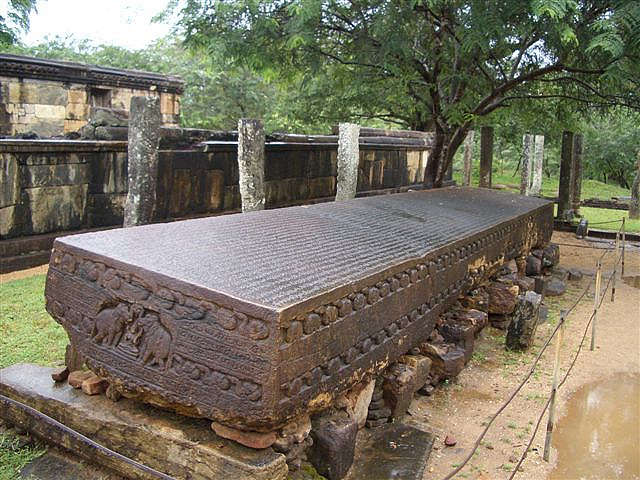
\includegraphics[width=.7\linewidth,trim=0 0 0 120pt,clip]{galpotha.jpeg}

  \smallskip

  A Sinhalese inscription, weighing 25 tonnes
\end{center}

The inscriptions are oft-times in a poor state, having been lying
around for a long time. Stones erode and break, and parts of the
inscriptions disappear, making the task of deciphering them a
fastidious and laborious one. Because of this, the archeologists'
guild has decided to climb on the IT train by commissioning an app
which, making use of the camera of a mobile device, both reads and
deciphers old inscriptions.

Image processing not really being your cup of tea, you have been
charged with the deciphering part of the app. To have an idea of the
task ahead of you, an example of a recently found inscription is shown
below.
\begin{center}
  \begin{minipage}{.6\linewidth}
\begin{verbatim}
as@@@mas e os baro@s assinalad@@
que @@ ocidental @@aia lusita@@
por m@@es nunca @@ antes nave@@@@@
passar@@ ainda al@@ da taproba@@
em pe@@gos e gue@@a@ esforcados
@ais @o que pr@@@ti@@a forca hum@@@
@ ent@e gent@@@emota@@dificaram
@ovo@reino @@e tanto @ublimaram
\end{verbatim}
  \end{minipage}
\end{center}
In this example text, the characters that could not be properly
identified have been replaced with the \texttt{@} (at) symbol.
% It is easy to notice that the stone where the text was engraved was,
% at some point, broken into several pieces, causing the characters
% along the cracks to become impossible to identify.

To be able to correctly decipher the inscription, the app must have
access to the vocabulary of the language of the text, which in this
case seems to be an archaic form of Portuguese, and then try to match
the text with it.


\subsection*{Task}

You are given the vocabulary of a language and a partially obfuscated
text. Your task is to write a program which checks whether it is
possible to transform each line into white space-separated words from
the given vocabulary, by putting one symbol from the alphabet of the
language or a white space in every place where the original symbol
could not be identified.

To simplify your task, all symbols from the original alphabet have
been mapped into the lower-case letters of the English alphabet.

Note that no text may contain two adjacent white spaces, and that no
line of text may start or end with a white space.


\subsection*{Input}

The program input consists of $1 + W + L$ lines.

The first line contains two white space-separated integers: the number
$W$ of words in the vocabulary, and the number $L$ of lines in the
inscription.

The following $W$ lines contain the vocabulary words, one per line.
Each word is a non-empty sequence of lower-case letters.

The remaining $L$ lines are the lines containing the transcript of the
inscription, each containing a non-empty sequence of lower-case
letters, white spaces, and \texttt{@} symbols. No line contains two
adjacent white spaces, or begins or ends with a white space.


\subsection*{Output}

The output will consist of $L$ lines, each one containing either the
word \texttt{yes} or the word \texttt{no}. If the $i^{th}$ line of the
inscription can be transformed into a sequence of words from the
vocabulary of the language, the $i^{th}$ line of the output will
contain the word \texttt{yes}, otherwise it will contain the word
\texttt{no}.


\subsection*{Constraints}

% (\emph{Optimistic constraints\ldots})

\begin{itemize}
\item $1 \le W \le 5000$
\item $1 \le L \le 40$
\end{itemize}
\begin{itemize}
\item The maximum word length is 20 characters.
\item The maximum line length is 70 characters.
\item The maximum number of consecutive \texttt{@} symbols is 10.
\end{itemize}


\subsection*{Input example 1}

\begin{verbatim}
3 16
ab
acb
baba
ab acb baba
a@ acb b@ba
ab@acb baba
a@@ac@@ba@@
@b @cb @aba
@b@@cb@@@ba
ba acb baba
b@ acb baba
ab acb baba@@
a
b
ba
b@
@ab
ab@
ab@@ab
\end{verbatim}

\subsection*{Output example 1}

\begin{verbatim}
yes
yes
yes
yes
yes
yes
no
no
no
no
no
no
no
no
no
no
\end{verbatim}


\subsection*{Input example 2}

\begin{verbatim}
39 8
a
que
os
mais
forca
assinalados
e
ainda
reino
passaram
mares
gente
baroes
edificaram
alem
remota
perigos
navegados
guerras
da
em
antes
sublimaram
por
novo
humana
de
entre
armas
tanto
praia
nunca
lusitana
do
esforcados
as
taprobana
prometia
ocidental
as@@@mas e os baro@s assinalad@@
que @@ ocidental @@aia lusita@@
por m@@es nunca @@ antes nave@@@@@
passar@@ ainda al@@ da taproba@@
em pe@@gos e gue@@a@ esforcados
@ais @o que pr@@@ti@@a forca hum@@@
@ ent@e gent@@@emota@@dificaram
@ovo@reino @@e tanto @ublimaram
\end{verbatim}

\subsection*{Output example 2}

\begin{verbatim}
yes
yes
yes
yes
yes
yes
yes
yes
\end{verbatim}

\end{document}
